
%-------------------------
% Resume in Latex
% Author : Sourabh Bajaj
% License : MIT
%------------------------

\documentclass[letterpaper,11pt]{article}

\usepackage{latexsym}
\usepackage[empty]{fullpage}
\usepackage{titlesec}
\usepackage{marvosym}
\usepackage[usenames,dvipsnames]{color}
\usepackage{verbatim}
\usepackage{enumitem}
\usepackage[pdftex]{hyperref}
\usepackage{fancyhdr}
\usepackage{zh_CN-Adobefonts_external}
\usepackage{graphicx}
\usepackage{multirow}


\pagestyle{fancy}
\fancyhf{} % clear all header and footer fields
\fancyfoot{}
\renewcommand{\headrulewidth}{0pt}
\renewcommand{\footrulewidth}{0pt}

% Adjust margins
\addtolength{\oddsidemargin}{-0.375in}
\addtolength{\evensidemargin}{-0.375in}
\addtolength{\textwidth}{1in}
\addtolength{\topmargin}{-.5in}
\addtolength{\textheight}{1.0in}

\urlstyle{same}

\raggedbottom
\raggedright
\setlength{\tabcolsep}{0in}

% Sections formatting
\titleformat{\section}{
  \vspace{-4pt}\scshape\raggedright\large
}{}{0em}{}[\color{black}\titlerule \vspace{-5pt}]

%-------------------------
% Custom commands
\newcommand{\resumeItem}[2]{
  \item\small{
    \textbf{#1}{: #2 \vspace{-2pt}}
  }
}

\newcommand{\resumeSubheading}[4]{
  \vspace{-1pt}\item
    \begin{tabular*}{0.47\textwidth}{l@{\extracolsep{\fill}}r}
      \textbf{#1} & #2 \\
      \textit{\small#3} & \textit{\small #4} \\
    \end{tabular*}\vspace{-5pt}
}

\newcommand{\resumeSubItem}[2]{\resumeItem{#1}{#2}\vspace{-4pt}}

\renewcommand{\labelitemii}{$\circ$}

\newcommand{\resumeSubHeadingListStart}{\begin{itemize}[leftmargin=*]}
\newcommand{\resumeSubHeadingListEnd}{\end{itemize}}
\newcommand{\resumeItemListStart}{\begin{itemize}}
\newcommand{\resumeItemListEnd}{\end{itemize}\vspace{-5pt}}

%-------------------------------------------
%%%%%%  CV STARTS HERE  %%%%%%%%%%%%%%%%%%%%%%%%%%%%


\begin{document}

%----------HEADING-----------------
\begin{tabular*}{0.8\textwidth}{l@{\extracolsep{\fill}}r}
    & \multirow{3}{4em}{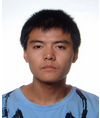
\includegraphics[height=3cm]{huizhu.png}} \\

    姓名 : 赵会铸 & \\

    出生年月: 1990.10 &\\

    邮箱 : zhaohuizhu@ruc.edu.cn & \\

    电话 : 180-0109-0187  & \\

    %github: \href{https://github.com/huizhuzhao}{https://github.com/huizhuzhao} & \\

    博客 \& github: \href{https://huizhuzhao.github.io/}{https://huizhuzhao.github.io} & \\

    应聘岗位:Machine Learning \& Data Science
\end{tabular*}

\section{教育}
\begin{itemize}
\item \textbf{中国人民大学} \qquad 理论物理专业 \qquad 硕士 \qquad 2012. 09 -- 2015. 07 \\
    %课程: 统计物理, 计算物理方法, 数学物理方法, 高等量子力学, 固体理论。

    北京市优秀硕士毕业生
    
    研究生国家奖学金

\item \textbf{河北工业大学} \qquad 工程管理专业 \qquad 本科 \qquad 2008. 09 -- 2012. 07 \\
    %课程: 管理学原理, 微观经济学, 运筹学, 项目风险管理, 土木工程。

    天津市大学生数学竞赛一等奖
    
    全国大学生数学竞赛赛区二等奖

    天津市大学生物理竞赛-拓普杯二等奖

\end{itemize}


\section{技能}
\begin{itemize}
\item 熟练掌握 python; 熟悉 C (研究生期间使用, 有MPI经验),  Linux 开发环境,git
\item 机器学习框架 : tensorflow, keras, theano, lasagne, sklearn; \quad 深度学习模型 LR, MLP, CNN, RNN
\item 英语 : TOEFL 93, GER: 322+3.0,良好的英语口语和阅读能力
\item 能够独立思考并承担研发任务,具有团队合作精神
\end{itemize}

\section{工作经历}

\begin{itemize}

\item 北京晶派科技有限公司 \qquad 算法工程师 (算法组负责人) \qquad 2016. 04 -- 现在

    主要负责将深度学习算法应用到药物设计领域; 包括利用生成模型(VAE)生成有效的分子库, 构建化学分子的定量构效关系 (QSAR) 模型,
    %进而对药物分子的各种物理化学性质进行预测; 
    蛋白质折叠以及蛋白质与药物分子之间的结合亲和力预测。
    
常用模型包括 MLP, CNN, RNN 等神经网络模型 (基于 tensorflow 和 theano) 和随机森林, 支持向量机等传统机器学习模型 (基于 sklearn)。


\item 星图数据 \qquad 数据分析师 \qquad 2015. 09 -- 2015. 11

参与数据爬取工作,即从各种电商平台爬取商品数据,并整理录入数据库。

\end{itemize}


\section{主要参与项目}
\begin{itemize}

\item 基于tensorflow的算法库

基于 tensorflow 实现了多种神经网络模型,并将模型的各个部分模块化,使之能够快速灵活的搭建出
最新的神经网络模型,并应用到不同的药物数据集上进行对照测试.

个人工作:负责 layers, metrics, optimizers 等模块,以及数据流模块 datasets

\item 分子数据预处理

化学分子通常以字符串和文件格式保存,数据预处理模块负责将各种数据源信息转化为矩阵形式进而供模型训练使用。

个人工作:基于 rdkit, openbabel (计算化学包) 构建 Molecule, Atom, Bond 等基础类对象,统一数据读取接口

%在构建各种机器学习模型之前,需要将分子数据进行矢量化操作将其转化成模型可读取的矩阵形式。
%通常做法是使用化学软件包生成分子描述符 (descriptor),但此方法得到的描述符仅在特定任务上表现较好,
%为了能够在不同任务上取得更好的结果,需要矢量化后的矩阵包含更为完整的分子信息,进而让模型自动提
%取针对特定任务的有效信息; 具体方法包括构建分子的库伦矩阵表示 (coulomb matrix), 化学键袋表示 (bag of bonds)
%(rdkit, openbabel, sklearn)

\item 图卷积神经网络模型 (参考文献 \href{https://arxiv.org/pdf/1509.09292.pdf}{paper})

该模型是监督式的机器学习模型,以分子的拓扑图为输入,对节点原子和连接键的信息进行图卷积,
经过多次迭代提取分子的特征表示,进而进行分类/回归任务的预测。该模型优于传统模型的地方在于
能够根据特定的任务提取最有效的特征表示,并且能够保证原子/键的排序不变性 (order-invariance),
因此具有较好的泛化能力。(tensorflow, lasagne)


\item 多任务学习模型(multitask neural net)

药物分子在不同靶点上的选择性是分子筛选重要的一方面,考虑到完整的实验数据较难获得,因此尝试多任务的学习模型来训练分子在 102 个靶点上的激活情况(active/inactive),这样通过不同任务之间分子数据的共享能够显著提高任务的预测准确率。

个人工作:基于 tensorflow 搭建多任务 (102) 的二分类模型,在百万规模的分子数据集上进行训练,单 GPU (1080) 训练时长约三天

%\item 自编码器模型

%新药设计的前期工作包括候选分子库的准备,该模型旨在通过变分自编码器生成有效的化学分子,并筛选出特定药物性质的候选者。

%模型以分子SMILES字符串(Simplified Molecular Input Line Entry Specification)为输入,第一步通过卷积/全连接操作将该离散的分子输入转换成连续向量 (encoder),
%并以该向量为输入预测分子的物化性质;第二步以该连续向量为输入通过 LSTM, GRU 进行反向编译输出分子 SMILES (decoder);
%通过修改连续向量得到具有较好物化性质的特征,进而使用decoder得出具有相应属性的分子结构。 (keras, tensorflow)

\item 靶点蛋白亲和力模型 (binding affinity)

新药设计的前期工作主要是从大量分子库中筛选出在靶点蛋白上有高活性的分子,进而推进到实验阶段。该模型的输入是复合物分子的结构数据,即药物分子+靶点蛋白的原子坐标,通过全连接网络进行图卷积从而对复合物之间的活性水平进行预测。模型在测试数据集上的表现优于传统的商业软件(schrodinger 等),目前我们筛选出的分子已经推进到酶实验阶段。

\item 全球人工智能黑客马拉松 (北京站)

该比赛为期两天 (2017.06.24-06.25),我们小组(主要有三名成员参与了比赛的全过程)的选题为人脸表情识别,训练数据集包含约7千张图片,
共分为7个类别(样本不均衡)。最终我们的算法 (VGG 模型) 以 57\%的准确率获得该选题的第一名。

个人工作:使用 keras 搭建分类模型 (\href{https://github.com/huizhuzhao/Hackthon}{code})

\end{itemize}

\section{论文发表}

\begin{itemize}
\item Deviation from the Maxwell-Cattaneo law: the role of the asymmetric interactions \\
Huizhu Zhao, Lei Wang \href{https://journals.aps.org/pre/abstract/10.1103/PhysRevE.92.042136}{Phys.Rev.E 92, 042136}
\item Heat-current correlation loss induced by finite-size effects in a one-dimensional nonlinear lattice \\
Lei Wang, Lubo Xu, Huizhu Zhao, \href{https://journals.aps.org/pre/abstract/10.1103/PhysRevE.91.012110}{Phys. Rev. E 91, 012110}
\end{itemize}


\section{自我介绍}

本人对机器学习领域有强烈的兴趣,有志于将先进的算法应用于各项业务以挖掘海量数据中隐藏的规律;
有较强的学习能力,能快速复现论文中的模型;
较强的团队合作意识,注重团队的学习氛围(论文阅读分享,code review,活跃的讨论),希望加入以业务为驱动的算法组,一起解决有挑战的技术难题。



\end{document}
